\documentclass[areasetadvanced]{scrartcl}

\usepackage[utf8]{inputenc}
\usepackage[T2A]{fontenc}
\usepackage[english,russian]{babel}

\usepackage[footskip=1cm,left=25mm, right=15mm, top=20mm, bottom=20mm]{geometry}
\usepackage{setspace}
\usepackage{amsmath, amssymb} 
\usepackage{graphicx}
\usepackage{tikz}
\usetikzlibrary{arrows.meta}
\usepackage{float}
\usepackage{dashrule}
\usepackage{fancyhdr} 
\usepackage{hyperref} 
\usepackage{parskip}
\usepackage{textcomp, enumitem}
\usepackage{indentfirst}
\usepackage{graphicx}
\usepackage{algorithm}
\usepackage{algpseudocode}
\usepackage{array} 
\usepackage{geometry}
\usepackage{afterpage}
\usepackage{minted}
\setcounter{secnumdepth}{3} 
\setcounter{tocdepth}{3}    
\usepackage{listings} 

\newcommand{\icon}[1]{\includegraphics[height=1.2em]{#1}}

\tikzstyle{block} = [rectangle, rounded corners, minimum width=3cm, minimum height=1cm, text centered, draw=black, fill=lightgray]

\setkomafont{sectioning}{\normalfont\bfseries} 
\setkomafont{section}{\normalfont\Large\bfseries}
\setkomafont{subsection}{\normalfont\large\bfseries}
\setkomafont{subsubsection}{\normalfont\large\bfseries}
\setkomafont{paragraph}{\normalfont\large\bfseries} 

\lstset{
  language=Haskell,
  basicstyle=\ttfamily\small,
  keywordstyle=\color{blue}\bfseries,
  stringstyle=\color{red},
  commentstyle=\color{green!70!black},
  numbers=left,
  numberstyle=\tiny,
  stepnumber=1,
  numbersep=10pt,
  showstringspaces=false,
  breaklines=true,
  frame=single
}

\lstdefinelanguage{Lua}{
    keywords={function, end, if, then, else, elseif, for, while, do, repeat, until, break, return, local, and, or, not, true, false, nil},
    keywordstyle=\color{blue}\bfseries,
    stringstyle=\color{red},
    commentstyle=\color{green!70!black},
    morestring=[s]{"}{"},
    morestring=[s]{'}{'},
    morecomment=[l]{--},
    morecomment=[s]{--[[}{]]},
    basicstyle=\ttfamily\small,
    numbers=left,
    numberstyle=\tiny,
    stepnumber=1,
    numbersep=10pt,
    showstringspaces=false,
    breaklines=true,
    frame=single
}

\setlength{\parindent}{1.25cm}
\setcounter{tocdepth}{2}
\begin{document}
\sloppy
	\thispagestyle{empty}
	\begin{center}
		\large{МИНОБРНАУКИ РОССИИ} \par
		\vspace{0.3cm}
		\normalsize
		{ФЕДЕРАЛЬНОЕ ГОСУДАРСТВЕННОЕ АВТОНОМНОЕ ОБРАЗОВАТЕЛЬНОЕ УЧРЕЖДЕНИЕ ВЫСШЕГО ОБРАЗОВАНИЯ} \par
		\vspace{0.3cm}
		\textbf{\guillemotleft САНКТ-ПЕТЕРБУРГСКИЙ ПОЛИТЕХНИЧЕСКИЙ}
		\textbf{УНИВЕРСИТЕТ ПЕТРА ВЕЛИКОГО\guillemotright} \par
		\vspace{0.3cm}
		{Институт компьютерных наук и кибербезопасности}\par
		{Высшая школа технологий искусственного интеллекта}\par
	\end{center}
	\vfill
	\begin{center}

        \par
		{\Huge РЕФЕРАТ}\par
        \large {на тему: \guillemotleft Муравьиный алгоритм построения пути\guillemotright}\par
		\Large {Дисциплина: Генетические алгоритмы}
	\end{center}
	\vfill
	\begin{flushleft}
		Студент: \hspace{1.8cm} \rule[0pt]{2.5cm}{0.5pt}\hfill Салимли Айзек Мухтар Оглы\par
		\vspace{1.5cm}
		Преподаватель: \hspace{0.55cm} \rule[0pt]{2.5cm}{0.5pt}\hfill  Большаков Александр Афанасьевич
	\end{flushleft}
	\vspace{0.5cm}
	\begin{flushright}
		\guillemotleft \rule[0pt]{0.8cm}{0.5pt}\guillemotright \rule[0pt]{2cm}{0.5pt} 20\rule[0pt]{0.5cm}{0.5pt} г.
	\end{flushright}
	\vfill
	\begin{center}
		Санкт-Петербург, 2025
	\end{center}
	\newpage
	\tableofcontents
	\newpage
	\newpage
	\section*{Введение}
	\addcontentsline{toc}{section}{Введение}
	Планирование пути мобильного робота является фундаментальной задачей автономной робототехники. Под задачей понимается вычисление траектории, которая переводит робота из заданной начальной позиции \(S\) в целевую позицию \(T\) в некотором рабочем пространстве, содержащем стационарные и/или подвижные препятствия. Критериями качества решения обычно являются: отсутствие столкновений, минимальная длина траектории, минимальное время движения, безопасность движения и соблюдение динамических ограничений робота.
	
	Рассматривается подход к планированию пути, основанный на муравьином алгоритме (Ant Colony System, ACS), а также его гибридные комбинации с классическими алгоритмами графового поиска и методами построения свободного пространства (MAKLINK). Муравьиный подход реализует стохастический многократный поиск, опирающийся на коллективную память в виде искусственного феромона. Этот подход является пригодным для задач с большой размерностью пространства и сложной структурой препятствий, поскольку демонстрирует хорошую способность находить качественные пути и быстро сходиться при корректной параметризации.
	
	Введение в проблематику включает следующие ключевые положения:
	\begin{itemize}
	  \item отличие статической (полностью известной) и динамической (частично неизвестной) среды и связанные с этим режимы планирования;
	  \item роль представления окружения (решётка/grid, MAKLINK-граф) для постановки дискретизированной задачи;
	  \item мотивация использования стохастических методов (МА) и комбинированных подходов (гибрид Дейкстра + МА) для повышения качества и надёжности путей.
	\end{itemize}
	
	\newpage
	\section{Постановка задачи}
	\subsection{Математическая формулировка}
	Пусть \(\mathcal{W}\) --- рабочее пространство робота, \(\mathcal{O}=\bigcup_{k} O_k\) --- множество областей препятствий. Требуется построить дискретизированную последовательность точек
	\[
	\mathcal{P} = \{P_0=S, P_1, \ldots, P_n=T\},
	\]
	такую, что для каждого сегмента:
	\[
	\operatorname{seg}(P_{i-1},P_i) \cap \mathcal{O} = \varnothing.
	\]
	Цель оптимизации может формулироваться, например, как минимизация длины пути:
	\[
	L(\mathcal{P}) = \sum_{i=1}^{n} \|P_i - P_{i-1}\| \quad \rightarrow \min.
	\]
	
	\subsection{Ограничения и требования}
	Задача планирования должна учитывать:
	\begin{itemize}
	  \item геометрические размеры и формы препятствий;
	  \item динамические ограничения робота (максимальная скорость, радиус разворота и т.п.), если они включены;
	  \item необходимость работы в статических и динамических условиях (т.е. возможность обработки новых препятствий, появляющихся в процессе движения);
	  \item требования к вычислительным затратам и числу итераций для получения решения в заданном времени.
	\end{itemize}
	
	\subsection{Ключевые подзадачи навигации}
	При решении общей задачи принято выделять четыре взаимосвязанные подзадачи:
	\begin{enumerate}
	  \item локализация робота в пространстве;
	  \item построение и обновление карты окружения;
	  \item планирование пути (поиск безопасной траектории);
	  \item управление движением (следование по траектории).
	\end{enumerate}
	В данной работе основной акцент делается на задаче (3) --- планировании пути.
	
	\newpage
	\section{Типы планирования пути}
	\subsection{Глобальное планирование (статическая среда)}
	Глобальное планирование предполагает, что всю информацию о среде (координаты и формы препятствий) можно задать заранее. Тогда задача решается следующим образом: строится полная модель пространства и на ней выполняется алгоритм поиска пути (например, на графе, полученном из сеточной дискретизации или из MAKLINK-графа). Глобальное планирование позволяет гарантировать отсутствие столкновений при условии корректности карты, и позволяет оптимизировать выбранный критерий (длина, время, и т.д.).
	
	\subsection{Локальное планирование (динамическая среда)}
	Локальное планирование применяется, когда среда частично неизвестна или динамична: новые препятствия могут появляться во время движения робота. В этом случае необходим режим online, в котором сенсоры робота периодически сообщают об обнаруженных препятствиях, и планировщик корректирует маршрут в реальном времени, сохраняя приоритет безопасности и корректности траектории.
	
	\subsection{Гибридный подход}
	Практически часто используется гибрид: глобальный план предоставляет ориентировочную траекторию, а локальный планировщик выполняет обработку неожиданных помех и корректирует движения. Гибридная схема сочетает надёжность глобального поиска и адаптивность локального управления.
	\begin{figure}[H]
		\centering
		\includegraphics[width=0.68\linewidth]{img/Screenshot 2025-11-01 at 00.03.43.png}
		\caption{Проблемы навигации робота}
	\end{figure}

	\newpage
	\section{Представление окружающей среды и модели}
	\subsection{Решётка (grid)}
	Один из простых способов моделирования --- разбить пространство на равномерную решётку клеток. Каждая клетка помечается как свободная или занятая. Путь затем рассматривается как последовательность переходов между центрами свободных клеток. Выбор разрешённого набора направлений движения определяет структуру графа:
	\begin{itemize}
	  \item 4-соседство: движения по горизонтали и вертикали;
	  \item 8-соседство: добавление диагональных переходов;
	  \item расширенные варианты: 16, 24, 30 направлений (увеличение степени свободы при выборе направления).
	\end{itemize}
	
	\subsection{MAKLINK-модель свободного пространства}
	MAKLINK-подход заключается в представлении свободного пространства через набор свободных линий, соединяющих вершины окаймлённых препятствий и границы среды. Основные этапы формирования модели:
	\begin{enumerate}
	  \item окаймление (расширение) границ препятствий для обеспечения безопасного буфера;
	  \item построение всех возможных линий, соединяющих углы окаймлённых препятствий;
	  \item удаление пересекающих препятствия или избыточных линий для формирования выпуклых областей свободного пространства;
	  \item взятие средних точек оставшихся свободных линий как вершин (узлов) MAKLINK-графа.
	\end{enumerate}
	Далее строится граф из средних точек; путём по этому графу (например, алгоритмом Дейкстры) находится субоптимальное безопасное решение, которое может служить начальным приближением для дальнейшей оптимизации.
			
	\begin{figure}[H]
		\centering
		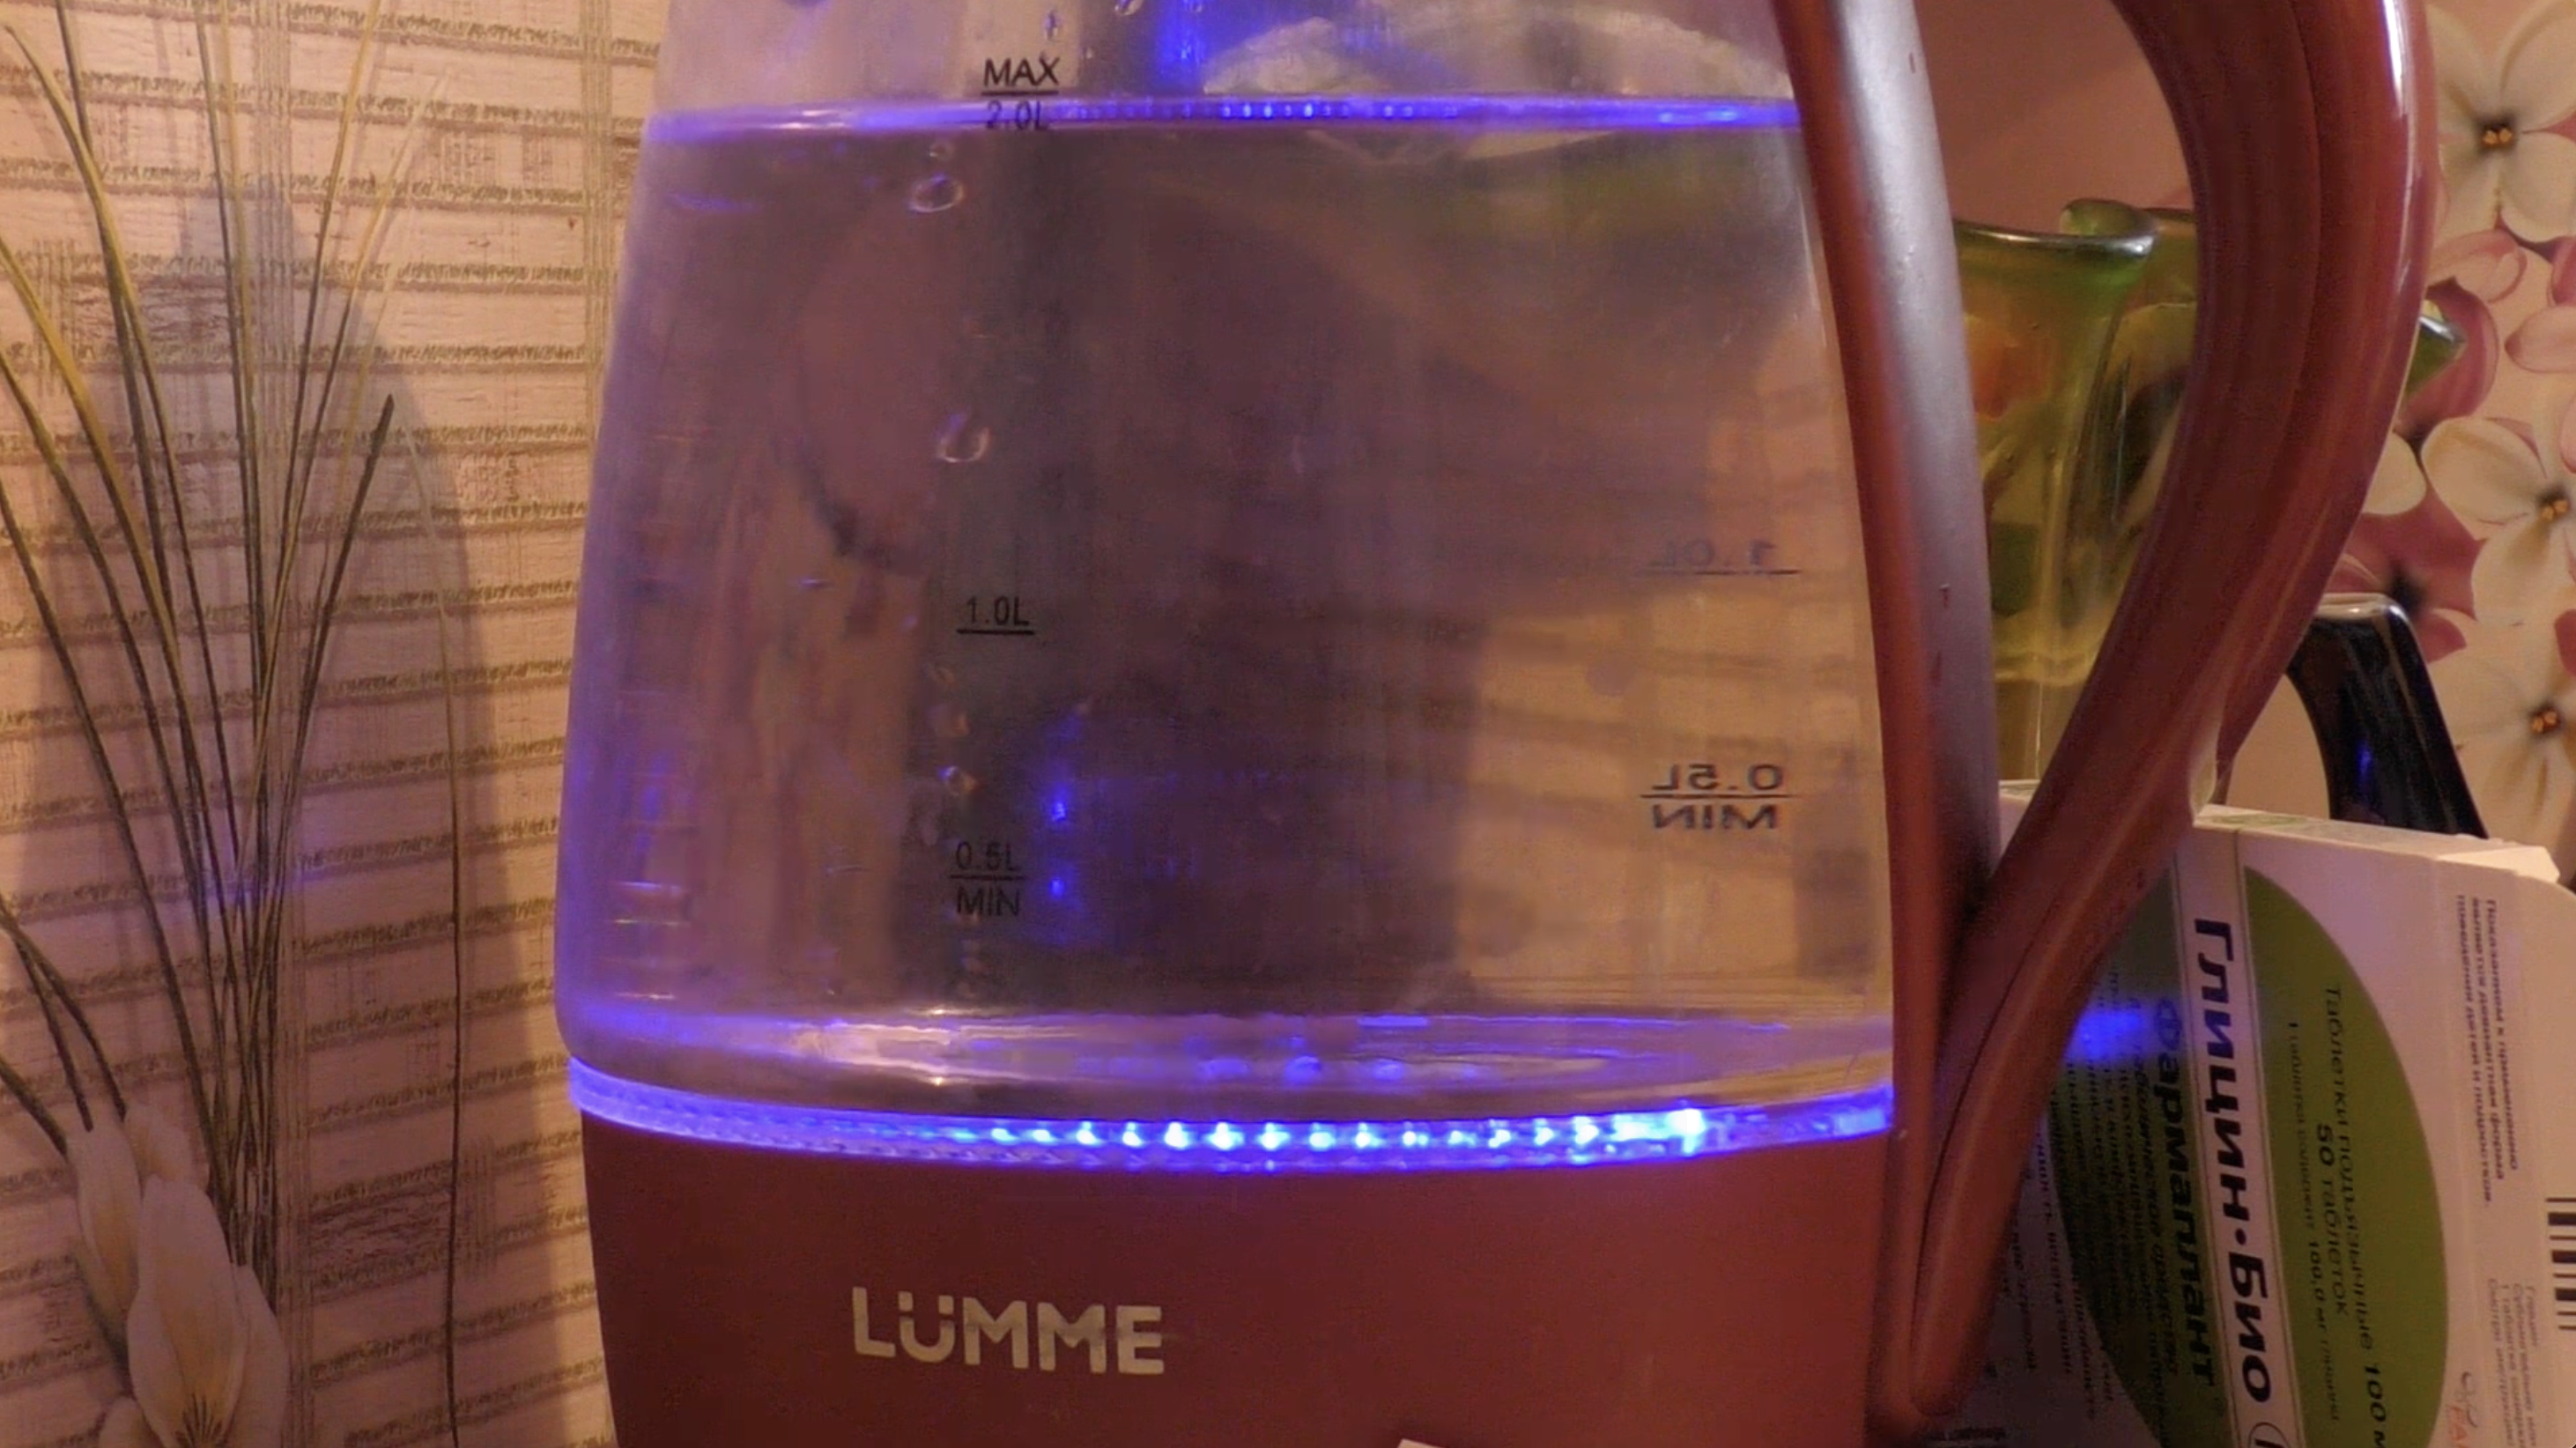
\includegraphics[width=0.74\linewidth]{img/image.png}
		\caption{MAKLINK граф: без избыточных свободных линий}
	\end{figure}

	\begin{figure}[H]
		\centering
		\includegraphics[width=0.74\linewidth]{img/image copy.png}
		\caption{MAKLINK граф: соединненые средние точки}
	\end{figure}
	
	\begin{figure}[H]
		\centering
		\includegraphics[width=0.74\linewidth]{img/image copy 2.png}
		\caption{MAKLINK граф: пути}
	\end{figure}
	
	\subsection{Преимущества и недостатки моделей}
	\begin{itemize}
	  \item Grid: простота реализации, гибкость, но возможна большая размерность и чувствительность к разрешению (размеру клетки).
	  \item MAKLINK: более компактное представление свободного пространства, гарантии отсутствия пересечений с препятствиями, подходящее для построения субоптимальных маршрутов, пригодных для последующей оптимизации.
	\end{itemize}

	\newpage
	\section{Муравьиный алгоритм: базовые принципы и интуиция}
	Муравьиный алгоритм моделирует коллективное поведение агентов, способных оставлять и считывать след в окружающей среде. В контексте планирования пути агент --- это виртуальный муравей, проходящий по дискретизированному графу. Каждый агент независимо генерирует путь от \(S\) к \(T\), причем вероятность выбора очередного шага зависит от накопленной информации (феромона) и локальной эвристики (видимости перехода). Коллективное поведение реализуется через два ключевых механизма:
	\begin{enumerate}
	  \item \textbf{испарение феромона} --- снижение значений \(\tau\) во времени, что предотвращает преждевременную конвергенцию и способствует исследованию;
	  \item \textbf{подкрепление лучших решений} --- увеличение \(\tau\) на ребрах/узлах, входящих в хорошие по качеству пути.
	\end{enumerate}
	В результате алгоритм способен балансировать между исследованием новых областей пространства и эксплуатацией накопленного знания о хороших траекториях.

	\newpage
	\section{Ant Colony System (ACS): формализация}
	\subsection{Правило выбора перехода}
	Пусть муравей в текущей вершине \(i\) рассматривает множество соседних вершин \(\mathcal{N}_i\), исключая временно запрещённые вершины из ``BlackList''. Для каждой допустимой вершины \(j\) задаются:
	\begin{itemize}
	  \item феромоновая метка \(\tau_{ij}(t)\);
	  \item эвристическая характеристика \(\eta_{ij}(t)\) (например, обратная длине перехода или функция, учитывающая изменение направления);
	  \item параметры \(\alpha\) и \(\beta\), задающие относительную важность \(\tau\) и \(\eta\).
	\end{itemize}
	Тогда вероятность перехода:
	\[
	P_{ij}(t) = \frac{[\tau_{ij}(t)]^\alpha [\eta_{ij}(t)]^\beta}{\sum_{k\in \mathcal{N}_i \setminus \text{BlackList}} [\tau_{ik}(t)]^\alpha [\eta_{ik}(t)]^\beta}.
	\]
	Практическая реализация иногда включает жадный выбор с вероятностью \(q_0\) (если случайное \(q<q_0\), используется наиболее вероятный переход; иначе --- случайный по распределению \(P_{ij}\)).
	
	\subsection{Локальное обновление феромона}
	После того как муравей проходит ребро \((i,j)\), выполняется локальная коррекция:
	\[
	\tau_{ij} \leftarrow (1-\rho)\,\tau_{ij} + \rho\,\tau_0,
	\]
	где \(\tau_0\) --- базовый уровень феромона, \(\rho\) --- локальный коэффициент. Локальное уменьшение феромона способствует расширению поиска, уменьшая склонность других агентов к немедленному следованию тем же связям.
	
	\subsection{Глобальное обновление феромона}
	По завершении всех туров текущей итерации определяется лучший путь длины \(L^+\). Для ребёр \( (i,j) \) принадлежащих этому пути производится глобальное обновление:
	\[
	\tau_{ij}(t+1) = (1-\rho)\,\tau_{ij}(t) + \frac{Q}{L^+},
	\]
	где \(Q\) --- константа, масштабирующая вклад феромона от лучшего пути. Таким образом, лучшие решения получают пропорциональное вознаграждение, обратное длине пути.
	
	\subsection{Критерии и останов}
	Алгоритм повторяет итерации до выполнения одного из критериев:
	\begin{itemize}
	  \item достижение предельного числа итераций \(NC\);
	  \item все муравьи построили один и тот же путь (сходимость);
	  \item достижение требуемого уровня качества решения.
	\end{itemize}
	
	\newpage
	\section{Параметры алгоритма и практическая настройка}
	\subsection{Основные параметры}
	\begin{description}
	  \item[\(\alpha\)] степень влияния феромона в правиле перехода;
	  \item[\(\beta\)] степень влияния эвристики \(\eta\);
	  \item[\(\rho\)] коэффициент испарения/локальной коррекции феромона;
	  \item[\(Q\)] количество феромона, вносимого лучшим муравьём;
	  \item[\(\tau_0\)] начальная концентрация феромона;
	  \item[\(m\)] число муравьёв (мощность популяции);
	  \item[\(NC\)] максимальное число итераций.
	\end{description}
	
	\subsection{Влияние параметров на поведение}
	\begin{itemize}
	  \item Повышение \(\alpha\) увеличивает влияние накопленного феромона и ускоряет эксплуатацию уже найденных путей. Чрезмерно большое \(\alpha\) может привести к преждевременной сходимости.
	  \item Повышение \(\beta\) увеличивает роль эвристики (локальная видимость), что стимулирует локально оптимальные решения.
	  \item Большое \(\rho\) ускоряет испарение феромона; при больших значениях поддерживается более сильное исследование.
	  \item Размер популяции \(m\) влияет на разнообразие решений: малое \(m\) может ограничить поиск, слишком большое --- увеличить вычислительные затраты.
	\end{itemize}
	
	\subsection{Экспериментальная настройка (пример)}
	Практический выбор параметров обычно производится эмпирически. В одном из примеров эффективными оказались значения (порядокный пример): \(NC=200\), \(m=10\), \(\tau_0=0.2\), \(\rho=0.85\), \(\beta=2\), \(q_0=0.1\), \(\alpha=1.0\). (Значения приведены как ориентир и зависят от конкретной постановки).
	
	\newpage
	\section{Применение к решению на дискретных MAKLINK-линиях}
	\subsection{Дискретная параметризация}
	Построение пути через средние точки MAKLINK-линий сводит геометрическую задачу к параметрической оптимизации. На каждой линии \(i\) средняя точка может быть смещена вдоль перпендикулярного направления в одном из дискретных шагов \(\{h_{i,0},\dots,h_{i,r_i}\}\). Тогда путь описывается вектором дискретных смещений \(\mathbf{h} = (h_1,\dots,h_d)\). Задача оптимизации --- найти \(\mathbf{h}^*\) минимизирующий длину пути \(L(\mathbf{h})\).
	
	\subsection{MA как оптимизатор в пространстве смещений}
	Варианты смещений трактуются как ``узлы'' для муравьёв: муравей в позиции \(i\) выбирает вариант \(u\in A_i\) с вероятностью
	\[
	P_{iu}(t) = \frac{[\tau_{iu}(t)]^\alpha [\eta_{iu}(t)]^\beta}{\sum_{v\in A_i} [\tau_{iv}(t)]^\alpha [\eta_{iv}(t)]^\beta}.
	\]
	Здесь \(\eta_{iu}\) может задаваться через отклонение координат по \(y\) (или другой оси), например:
	\[
	\eta_{iu} = \frac{1}{1 + |y_{iu} - y_{iu}^*|},
	\]
	где \(y_{iu}^*\) — эталонное значение (например, по предыдущей итерации). Такой выбор \(\eta\) стремится к смещениям, приближающимся к ранее найденным хорошим решениям.
	
	\subsection{Алгоритмическая схема}
	В данной постановке один тур муравьиного алгоритма --- это продвижение всех \(m\) муравьёв от \(S\) по всем MAKLINK-линиям до \(T\), с записью выбранных смещений в массивы Path\(_k\) и локальными обновлениями \(\tau\). Затем вычисляются длины полученных путей \(L_k\), выбирается лучший \(L^+\) и выполняется глобальное обновление феромона. Далее возможна проверка на сходимость и повтор итераций.
	
	\newpage
	\section{Псевдокод детального алгоритма (шаги)}
	Ниже приведена формальная последовательность шагов алгоритма (развёрнутая версия):
	\begin{enumerate}
	  \item Построить MAKLINK-граф и найти субоптимальный путь \(S \to P_1 \to \dots \to P_d \to T\) методом Дейкстры.
	  \item Задать параметры: \(m, \tau_0, \rho, \alpha, \beta, q_0, NC\).
	  \item Инициализировать \(t \leftarrow 1\); для всех узлов установите \(\tau_{iu}=\tau_0\).
	  \item Поместить \(m\) муравьёв в начальную точку \(S\).
	  \item Для \(i=1\) до \(d\): для каждого муравья \(k=1\ldots m\):
		\begin{enumerate}
		  \item выбрать узел \(u\in A_i\) по правилу \(P_{iu}(t)\) (включая возможный жадный выбор при \(q<q_0\));
		  \item запомнить выбор в Path\(_k[i]\);
		  \item выполнить локальную коррекцию \(\tau_{iu} \leftarrow (1-\rho)\tau_{iu} + \rho\tau_0\).
		\end{enumerate}
	  \item После прохождения всех линий получить у каждого муравья геометрию пути \(P_1^k,\dots,P_d^k\) и вычислить длину \(L_k\).
	  \item Определить \(L^+=\min_k L_k\) и соответствующий путь \(T_t\). Обновить глобальную память: для всех рёбер/узлов, входящих в \(T_t\), выполнить \(\tau_{ij}(t+1) = (1-\rho)\tau_{ij}(t) + \frac{Q}{L^+}\).
	  \item Проверить условие остановки: если \(t\ge NC\) или все муравьи построили одинаковый путь, либо иное условие — завершить; иначе \(t\leftarrow t+1\) и вернуться к шагу 5.
	\end{enumerate}
	
	\newpage
	\section{Эксперименты и численные примеры}

	\textbf{Эксперемент был взят из методического материала$^{[1]}$}. Тестирование проводилось на наборах сред разной сложности: простая, относительно сложная, сложная. Проводились эксперименты с различными начальными и конечными точками, а также с разной конфигурацией препятствий.
	
	\paragraph{Примеры результатов}
	\paragraph{Пример 1 (сложная среда):}
	Начальная точка \(S=(5,50)\), целевая \(T=(400,450)\). Полученные длины маршрутов:
	\[
	L_{\text{MA}} = 913.82\ \text{см}.
	\]
	Для сравнения, генетический алгоритм на тех же данных дал:
	\[
	L_{\text{GA}} = 921.03\ \text{см}.
	\]
	Таким образом, МА показал лучшее качество пути в представленном тесте.
	
	\paragraph{Гибридный пример (MAKLINK + Дейкстра + МА):}
	\begin{itemize}
	  \item Субоптимальный путь (Дейкстра): \(L = 507.692\ \text{м}\).
	  \item После оптимизации МА: \(L = 440.233\ \text{м}\).
	  \item При увеличении точности дискретизации (более мелкий шаг \(h_i\)): \(L = 439.372\ \text{м}\).
	\end{itemize}
	Данные демонстрируют значительное улучшение качества пути после применения МА к субоптимальному начальному решению.
	
	\paragraph{Сходимость и сравнение по времени}
	В приведённых экспериментах:
	\begin{itemize}
	  \item МА достигает оптимума примерно на 38-й итерации;
	  \item ГА даёт оптимум примерно на 240-й итерации;
	  \item МА требует меньшее время на построение пути при равной мощности популяции.
	\end{itemize}
	
	\begin{figure}[H]
		\centering
		\includegraphics[width=0.44\linewidth]{img/Screenshot 2025-11-01 at 00.16.56.png}
		\caption{Результаты проведения анализа (с методического материала)}
	\end{figure}

	\begin{figure}[H]
		\centering
		\includegraphics[width=0.64\linewidth]{img/Screenshot 2025-11-01 at 00.17.11.png}
		\caption{Муравьиный алгоритм - дает оптимум на 38 итерации}
	\end{figure}

	\begin{figure}[H]
		\centering
		\includegraphics[width=0.64\linewidth]{img/Screenshot 2025-11-01 at 00.17.16.png}
		\caption{Генетический алгоритм - дает оптимум на 240 итерации}
	\end{figure}

	\begin{figure}[H]
		\centering
		\includegraphics[width=0.64\linewidth]{img/image copy 3.png}
		\caption{Сравнения отклонений}
	\end{figure}

	\newpage
	\section{Анализ влияния числа направлений движения}
	\subsection{Стандартные случаи}
	При 4 направлениях движение ограничено осями, при 8 направлениях добавляются диагонали, что обычно даёт лучшие пути и большую гибкость выбора.
	
	\subsection{Расширенные варианты и их эффект}
	Увеличение числа допустимых направлений до 16, 24 или 30 позволяет роботу выбирать более плавные и короткие траектории, но:
	\begin{itemize}
	  \item увеличивается количество возможных переходов из узла, что повышает вычислительную сложность расчёта вероятностей;
	  \item для МА это означает расширение множества альтернатив, что может увеличивать время на сходимость, но при правильно настроенных параметрах повышает шансы найти более качественное решение.
	\end{itemize}
	\begin{figure}[H]
		\centering
		\includegraphics[width=0.74\linewidth]{img/image copy 4.png}
		\caption{Сравнение по времени}
	\end{figure}

	\newpage
	\section{Гибридные подходы и преимущества интеграции методов}
	\subsection{Мотивы для гибрида}
	Комбинация детерминированных методов поиска (например, Дейкстра) с стохастическими оптимизаторами (МА) даёт:
	\begin{itemize}
	  \item гарантированный начальный путь без пересечений с препятствиями;
	  \item возможность улучшить начальное решение по качеству (длина, гладкость) за счёт стохастического поиска в локальном окне;
	  \item снижение риска попадания в локальные минимумы благодаря стохастическому исследованию.
	\end{itemize}
	
	\subsection{Описание примерной схемы}
	\begin{enumerate}
	  \item Построить MAKLINK-граф и найти субоптимальный путь алгоритмом Дейкстры.
	  \item Дискретизовать окрестности средних точек линий (возможные смещения).
	  \item Запустить МА для оптимизации вектора смещений.
	  \item По завершении получить оптимизированный путь и при необходимости выполнить сглаживание.
	\end{enumerate}
	
	\subsection{Числовые примеры эффективности}
	Ранее приведённые численные данные (спад длины с 507.692\,м до 440.233\,м) показывают, что гибридный подход может давать значительное улучшение качества решения.
	
	\subsection{Пример свободного пространства}
	Рассматривается дискретная сетка, которая представляет окружение робота, где Черным отмечены препятствия, белым свободные клетки, желтым отмечены вершины, которые может пересекать робот.
	\begin{figure}[H]
		\centering
		\includegraphics[width=0.74\linewidth]{img/image copy 5.png}
		\caption{Дискретная сетка}
	\end{figure}

	\begin{figure}[H]
		\centering
		\includegraphics[width=0.74\linewidth]{img/image copy 6.png}
		\caption{Простая карта свободного пространства}
	\end{figure}

	\begin{figure}[H]
		\centering
		\includegraphics[width=0.74\linewidth]{img/image copy 8.png}
		\caption{Средняя карта свободного пространства}
	\end{figure}

	\begin{figure}[H]
		\centering
		\includegraphics[width=0.74\linewidth]{img/image copy 7.png}
		\caption{Сложная карта свободного пространства}
	\end{figure}

	\newpage
	\section*{Заключение}
	\addcontentsline{toc}{section}{Заключение}
	\begin{itemize}
	  \item муравьиный алгоритм (ACS) является эффективным стохастическим методом для задачи планирования пути, демонстрирующим хорошую сходимость и качество решений на тестовых средах;
	  \item гибридные схемы, комбинирующие детерминированные алгоритмы (Дейкстра, MAKLINK) и МА, дают значительное улучшение начальных субоптимальных решений и обеспечивают безопасность (отсутствие столкновений);
	  \item корректная настройка параметров (\(\alpha,\beta,\rho,Q,m,NC\)) и выбор представления пространства (grid/MAKLINK) критично влияют на производительность и качество;
	  \item практические реализации должны учитывать динамику среды, интеграцию с сенсорными данными и требования к сглаживанию траекторий.
	\end{itemize}
	
	Рекомендуется использовать гибридный подход в задачах, где требуется сочетание гарантии отсутствия столкновений и высокого качества пути: построить субоптимальный безопасный маршрут детерминированно и затем улучшить его стохастическим оптимизатором (МА), при этом применяя адаптивную дискретизацию и параллельные вычисления для ускорения работы.
	\newpage
	\addcontentsline{toc}{section}{Список литературы}
	\begin{thebibliography}{9}

		\bibitem{dorigo1996}
		Скобцов Ю. А. 
		ГА: Планирование пути МА.  
		СПбПУ. 1-59 с.
		
		\bibitem{dorigo2006}
		DORIGO, M., BIRATTARI, M., STÜTZLE, T. 
		Ant Colony Optimization. 
		\textit{IEEE Computational Intelligence Magazine}. 
		2006. Vol. 1, no. 4. pp. 28–39.
		
		\bibitem{malgina}
		МАЛЬГИНА, Майя. 
		Графы и муравьиные алгоритмы. 
		\textit{Skillbox Media}. 
		Доступно по ссылке: https://skillbox.ru/media.
		
		\bibitem{tsurikov}
		ЦУРИКОВ, А. 
		Построение маршрутов с использованием муравьиных алгоритмов. 
		Доступно по ссылке: https://example.com.
		
		\bibitem{amazon}
		Amazon Robotics. 
		Применение муравьиных алгоритмов в логистике. 
		[Электронный ресурс]. 
		Доступно по ссылке: https://example.com/amazon.
		
		\bibitem{vasiliev2015}
		ВАСИЛЬЕВ, С. В., ПЕТРОВ, А. А. 
		Моделирование свободного пространства с использованием теории MAKLINK. 
		\textit{Известия вузов. Технические науки}. 
		2015. №3. С. 56–64.
		
		\bibitem{acs1997}
		ACS Ant Colony System: A new heuristic optimization approach for solving TSP. 
		\textit{Elsevier Science}. 
		1997. Vol. 6, no. 4. pp. 321–333.
		
		\bibitem{fedex}
		FedEx Logistics. 
		Оптимизация маршрутов на основе муравьиных алгоритмов. 
		[Электронный ресурс]. 
		Доступно по ссылке: https://example.com/fedex.
		
		\bibitem{bonabeau1999}
		BONABEAU, E., DORIGO, M., THERAULAZ, G. 
		Swarm Intelligence: From Natural to Artificial Systems. 
		\textit{Oxford University Press}. 1999.
		
		\end{thebibliography}
\end{document}